\documentclass[t,xcolor=pdftex,dvipsnames,table]{beamer}
\usepackage[]{graphicx}\usepackage[]{color}
%% maxwidth is the original width if it is less than linewidth
%% otherwise use linewidth (to make sure the graphics do not exceed the margin)
\makeatletter
\def\maxwidth{ %
  \ifdim\Gin@nat@width>\linewidth
    \linewidth
  \else
    \Gin@nat@width
  \fi
}
\makeatother

\definecolor{fgcolor}{rgb}{0.345, 0.345, 0.345}
\newcommand{\hlnum}[1]{\textcolor[rgb]{0.686,0.059,0.569}{#1}}%
\newcommand{\hlstr}[1]{\textcolor[rgb]{0.192,0.494,0.8}{#1}}%
\newcommand{\hlcom}[1]{\textcolor[rgb]{0.678,0.584,0.686}{\textit{#1}}}%
\newcommand{\hlopt}[1]{\textcolor[rgb]{0,0,0}{#1}}%
\newcommand{\hlstd}[1]{\textcolor[rgb]{0.345,0.345,0.345}{#1}}%
\newcommand{\hlkwa}[1]{\textcolor[rgb]{0.161,0.373,0.58}{\textbf{#1}}}%
\newcommand{\hlkwb}[1]{\textcolor[rgb]{0.69,0.353,0.396}{#1}}%
\newcommand{\hlkwc}[1]{\textcolor[rgb]{0.333,0.667,0.333}{#1}}%
\newcommand{\hlkwd}[1]{\textcolor[rgb]{0.737,0.353,0.396}{\textbf{#1}}}%
\let\hlipl\hlkwb

\usepackage{framed}
\makeatletter
\newenvironment{kframe}{%
 \def\at@end@of@kframe{}%
 \ifinner\ifhmode%
  \def\at@end@of@kframe{\end{minipage}}%
  \begin{minipage}{\columnwidth}%
 \fi\fi%
 \def\FrameCommand##1{\hskip\@totalleftmargin \hskip-\fboxsep
 \colorbox{shadecolor}{##1}\hskip-\fboxsep
     % There is no \\@totalrightmargin, so:
     \hskip-\linewidth \hskip-\@totalleftmargin \hskip\columnwidth}%
 \MakeFramed {\advance\hsize-\width
   \@totalleftmargin\z@ \linewidth\hsize
   \@setminipage}}%
 {\par\unskip\endMakeFramed%
 \at@end@of@kframe}
\makeatother

\definecolor{shadecolor}{rgb}{.97, .97, .97}
\definecolor{messagecolor}{rgb}{0, 0, 0}
\definecolor{warningcolor}{rgb}{1, 0, 1}
\definecolor{errorcolor}{rgb}{1, 0, 0}
\newenvironment{knitrout}{}{} % an empty environment to be redefined in TeX

\usepackage{alltt}
\newcommand{\SweaveOpts}[1]{}  % do not interfere with LaTeX
\newcommand{\SweaveInput}[1]{} % because they are not real TeX commands
\newcommand{\Sexpr}[1]{}       % will only be parsed by R


%\documentclass[handout,t,xcolor=pdftex,dvipsnames,table]{beamer}  % For handout
\mode<presentation>{
\useoutertheme[subsection=false]{miniframes}
%\beamertemplatenavigationsymbolsempty
\usecolortheme{custom}
\usefonttheme[onlymath]{serif}
\setbeamercovered{invisible}
%\setbeamertemplate{navigation symbols}{}
%\setbeamertemplate{mini frames}{}  % Old one
% Comment out this line to give the header
% \setbeamertemplate{headline}[default]
\setbeamertemplate{caption}[numbered]
%\setbeamertemplate{itemize items}[circle] 
\setbeamertemplate{frametitle continuation}{\frametitle{\color{white}Title}}  % So no tile on subsequent frames, from [allowframebreaks]

%%% CUSTOMISING NAVIATION %%%%
%This customises the navigation to be thin width and just have section headings (not subsections). 
\setbeamertemplate{headline}{%
\leavevmode%
  \hbox{%
    \begin{beamercolorbox}[wd=\paperwidth,ht=2.5ex,dp=1.125ex]{palette tertiary}%   % Tertiary colour is blue
    \insertsectionnavigationhorizontal{\paperwidth}{}{\hskip0pt plus1filll}
    \end{beamercolorbox}%
}}}

\RequirePackage{marvosym}

%%% INCLUDING SOLUTIONS %%%%
%% You can incorporate both questions and solutions in the 
%% same document.  Solutions can be included between the 
%% commands \begin{soln} and \end{soln}
%% To generate a pdf with only the questions uncomment:
%\excludecomment{soln}
\usepackage{comment}
\specialcomment{soln}{\begingroup \vspace{1mm} \sl}{ \leavevmode \endgroup}

%%%% DETAILS FOR PART 1 TITLE PAGE (OLD) %%%%
%\title{\large Part2 - Probability \& Distribution Theory} 
%\subtitle{} 
%\author{\copyright Dr Di Warren 2016} 
%\date{MATH1005 - Statistics}
% \colorlet{Faculty}{Arts}
%\colorlet{Faculty}{MasterBrandRed} % This is only needed if the notes are used for different faculties.
%\colorlet{FacultyText}{White}
% Defines the color of the text used on the title page and ``blocks''
% White for Business; TitlePageBlack for Arts, Pharmacy and Science
%\definecolor{CoolBlack}{rgb}{0.0, 0.18, 0.39}

%%%% DETAILS FOR FULL COURSE TITLE PAGE %%%%
\title{\Huge STATISTICS} 
\subtitle{} 
\author{\copyright University of Sydney 2017 (Di Warren)} 
\date{MATH1005}
% \colorlet{Faculty}{Arts}
\colorlet{Faculty}{MasterBrandRed} % This is only needed if the notes are used for different faculties.
\colorlet{FacultyText}{White}
% Defines the color of the text used on the title page and ``blocks''
% White for Business; TitlePageBlack for Arts, Pharmacy and Science
\definecolor{CoolBlack}{rgb}{0.0, 0.18, 0.39}

%%%% PACKAGES %%%%
\usepackage{multirow}
\usepackage{fancybox}
\usepackage[english]{babel}
\usepackage[utf8]{inputenc}
\usepackage{bm}
\usepackage{array}
\usepackage{booktabs}
\usepackage{tikz}
\usetikzlibrary{matrix,arrows,decorations.pathmorphing}
\usepackage{verbatim}
\usepackage{pgf,pgfsys,pgffor}
\usepackage{pgfplots}
\pgfplotsset{compat=1.3} %Recommended as of Pgfplots 1.3 - necessary?
\usetikzlibrary{decorations.pathreplacing,calc}
\usetikzlibrary{shapes, backgrounds}   % For Venn diagrams
\def \setA{ (0,0) circle (1cm) }
\def \setB{ (1.5,0) circle (1cm) }
\def \setC{ (0.6,1.5) circle (1cm) }
\def \setO{ (-2, -1.5) rectangle (3.5, 2.75) }
\tikzstyle{every picture}+=[remember picture]
\tikzstyle{na} = [baseline=-.5ex]
\usepackage{listings}  %Added by Di for adding R code

%\AtBeginSection[]
%{
%   \begin{frame}
 %      \frametitle{Outline}
 %      \tableofcontents[currentsection]
%   \end{frame}
%}  %This seems overkill for weekly lecture slides.

%\AtBeginSection[]
%{
%  \begin{frame}
% \frametitle{Contents}
%  \tiny{\tableofcontents[currentsection]}
%  \end{frame}
%}
%\useoutertheme{infolines} % Just lists current section in navigation at top, nice but limiting?

%%%% TITLE PAGE AND CONTENTS AT BEGINNING OF EACH TOPIC %%%%

\RequirePackage{ifthen} % package required
\newboolean{sectiontoc}
\setboolean{sectiontoc}{true} %default to true

\AtBeginSection[]
{
\begin{frame}[plain]
\vspace{60pt}
\begin{center}
\Huge{{\textcolor{MasterBrandBlue} \insertsection}}
\end{center}
\begin{tikzpicture}[scale=0.54]
%\hspace{-12pt}
%% Big Rectangle
\fill[MasterBrandRed] (0,14) -- (20,14) -- (20,15) -- (0,15);

%\draw (1,14.5) node [anchor = west] {\textcolor{MasterBrandBlue}{\Huge{\insertsection}}}; Overlays box with title, but long titles drop off the page
\end{tikzpicture} 
\end{frame}

%%%%%WORKING VERSION OF TOC%%%%%
%\begin{frame}
%   \frametitle{Outline}
%  \tableofcontents[currentsection, sectionstyle=show/hide, subsectionstyle=show/show/hide]
%  \end{frame}
%}

%%%%%2 VERSIONS - WITH AND WITHOUT TOC%%%%%
  \ifthenelse{\boolean{sectiontoc}}{
    \begin{frame}
  \frametitle{Outline}
  \tableofcontents[currentsection, sectionstyle=show/hide, subsectionstyle=show/show/hide]
 \end{frame}
  }
}
%%%%%This doesnt seem to work?%%%%
\newcommand{\toclesssection}[1]{
  \setboolean{sectiontoc}{false}
  %\section{#1}
  \setboolean{sectiontoc}{true}
}


% PDF settings
%\hypersetup{%
%  pdftitle={\inserttitle \insertsubtitle},%
%  pdfauthor={Di Warren},%
%	pdfsubject={},%
%	pdfkeywords={}%   
%	 }

%%%%  HELPFUL MACROS %%%%
\newcommand{\ud}{\mathrm{d}}
\newcommand{\var}{\mathrm{var}}
\newcommand{\ep}{\varepsilon}
\newcommand{\cov}{\mathrm{cov}}
\newcommand{\tr}{\mathrm{tr}}
\newcommand{\MSE}{\mathrm{MSE}}
\newcommand{\rank}{\mathrm{rank}}
\newcommand{\Bias}{\mathrm{Bias}}
\newcommand{\dei}{\partial}
\newcommand{\E}{\mathbb{E}}
\newcommand{\N}{\mathcal{N}}
\newcommand{\bbR}{\mathbb{R}}
\newcommand{\V}{\mathbb{V}}
\newcommand{\betahat}{\hat{\beta}}
\newcommand{\CLRM}{$\mathbf{y} = X\bm{\beta} + \bm{\ep}$}

%%%% LOGO FOR SLIDES %%%%
\logo{\vspace{79mm}
\includegraphics[height=0.9cm]{../images/sydney.pdf}}

%%%% ADD PAGE NUMBER %%%%
\setbeamertemplate{sidebar right}{}
\setbeamertemplate{footline}{%
\hfill\usebeamertemplate***{navigation symbols}
\hspace{1cm}\insertframenumber{}/\inserttotalframenumber}

%%%% BEGIN CONTENT %%%


\begin{document}




%%%% TOPIC11 %%%%
\section[11]{Topic11: Test for Goodness of Fit (Chi-squared Test)}


\subsection[GoodnessofFit]{Example1: Mendel's Early Genetics Model}
\begin{frame}{Example1: Mendel's Early Genetics Model}

Mendel did much work in early genetics in the 19th Century, but it wasn't appreciated until later. He conducted experiments on the distributions of traits in pea plants. In one experiment, he classified 556 peas according to shape (Round or Angular) and colour (Yellow or Green). He predicted that the 4 different `offspring' (RY, RG, AY, AG) would occur in the ratio 9:3:3:1. He observed counts of 315, 108, 101 and 32. 

\vspace{.5cm}
{\bf Does Mendel's theory fit the data?}

\end{frame}

\subsection[GoodnessofFit]{Example2: Random Number Generator}
\begin{frame}[fragile]{Example2: Random Number Generator}
Suppose a Random Number Generator is being tested. 1000 values yield the following results. \\

\vspace{.5cm}
{\tiny 
\begin{tabular}{l|llllllll}  \hline
Cat. & [0,0.1) &  [0.1,0.2) & [0.2,0.3) & [0.3,0.4) & [0.4,0.5) & [0.5,0.6) & [0.6,0.7) & [0.7,0.8)  \\ \hline
$O_{i}$ & 136 & 105 & 107 & 89 & 97 & 84 & 76 & 84    \\ \hline
\end{tabular}
}

\vspace{.5cm}
{\tiny 
\begin{tabular}{l|lll}  \hline
Cat. & [0.8,0.9) &  [0.9,1] & Total \\ \hline
$O_{i}$ & 105  & 117  & 1000      \\ \hline
\end{tabular}
}

\vspace{.5cm}
{\bf Test the goodness of fit of the U[0,1] model to these counts.}

\begin{knitrout}
\definecolor{shadecolor}{rgb}{0.969, 0.969, 0.969}\color{fgcolor}
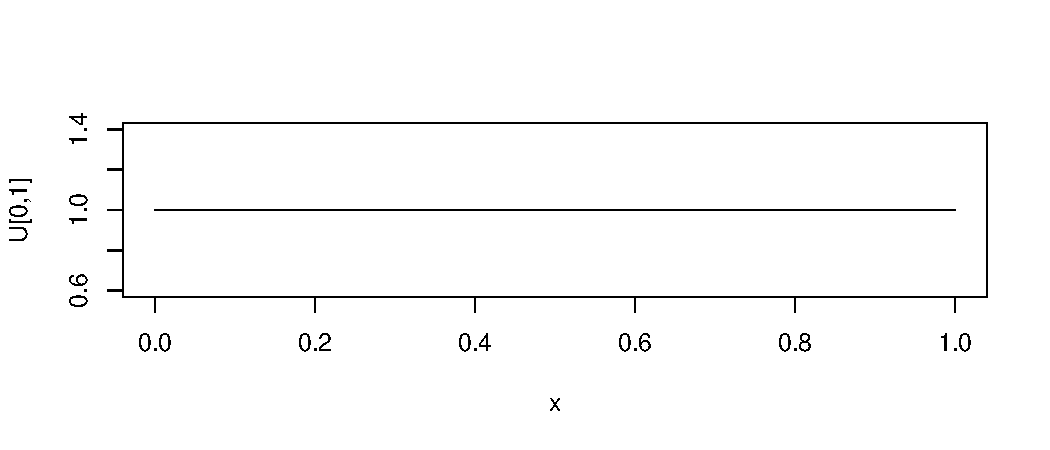
\includegraphics[width=\maxwidth]{figure/unnamed-chunk-2-1} 

\end{knitrout}
\end{frame}

\subsection[GoodnessofFit]{Example3: Testing Data fits a Binomial Model}
\begin{frame}[fragile]{Example3: Testing Data fits a Binomial Model}
Data results in the following frequency table and plot. \\

\vspace{.5cm}
\begin{tabular}{l|lllll} 
Category & 0 & 1 & 2 & 3 & Total  \\ \hline
$O_{i}$ & 19 & 34 & 27 & 20 & 100    \\ \hline
\end{tabular}

\begin{knitrout}
\definecolor{shadecolor}{rgb}{0.969, 0.969, 0.969}\color{fgcolor}
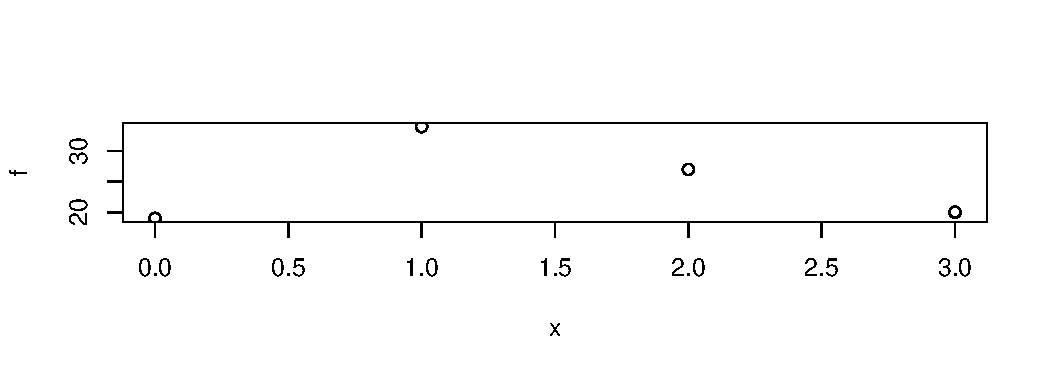
\includegraphics[width=\maxwidth]{figure/unnamed-chunk-3-1} 

\end{knitrout}

{\bf Test whether the data could be modelled by $Bin(n,p)$ for some $p$.}
\end{frame}

\begin{frame}
Putting this example into context, imagine a sports journalist claims that Michael Jordan's free throws follow a Binomial distribution with probability 80\%.
\href{https://sahilmohnani.wordpress.com/tag/binomial/}{\beamergotobutton{Sports Example}}
\href{https://www.youtube.com/watch?v=3lt1x-k3QGU}{\beamergotobutton{Larry Bird highlights}}

\end{frame}


\subsection[GoodnessofFit]{Example4: Testing Data fits a Normal Model}
\begin{frame}[fragile]{Example4: Testing Data fits a Normal Model}
Data results in the following histogram. \\



\includegraphics[height=4cm]{../images/Topic11_Q2.pdf}

\vspace{.5cm}
{\bf Test whether the following histogram could be modelled by a Normal distribution $N(\mu, \sigma^2)$?}
\end{frame}

\subsection[GoodnessofFit]{Interesting Facts about the Chi-Squared Distribution}

\begin{frame}[fragile]{Interesting Facts about the Chi-Squared Distribution}

For the Goodness of Fit test, we are going to use the 
Chi-Squared Distribution. Recall from Chapter 5:

\begin{definition}[Chi-Squared distribution]
The \alert{Chi-Squared distribution} is the sum of squared independent Standard Normal random variables $Z_{i} \sim N(0,1)$ $i=1,2,\ldots,n$. It can only take positive values and is typically right skewed.

\vspace{.5cm}
We say the variable $X = \sum_{i=1}^{n} Z_{i}^2 \sim \chi^2_{n}$ with $n$ degrees of freedom, and mean $E(X)=n$ and  variance $Var(X) = 2n$.

\vspace{.5cm}
The pdf is:
\[ f(x)  =  \frac{ 1}  { 2^{\frac{n}{2}} \Gamma(\frac{n}{2})}
x^{\frac{n}{2}-1} e^{-\frac{x}{2}}
\;\;\;\;\; \mbox{for }  x \in (0, \infty) \]

\end{definition}
\href{https://www.youtube.com/watch?v=hcDb12fsbBU}{\beamergotobutton{Link}}

\end{frame}

\begin{frame}[fragile]\frametitle{}
\begin{knitrout}
\definecolor{shadecolor}{rgb}{0.969, 0.969, 0.969}\color{fgcolor}
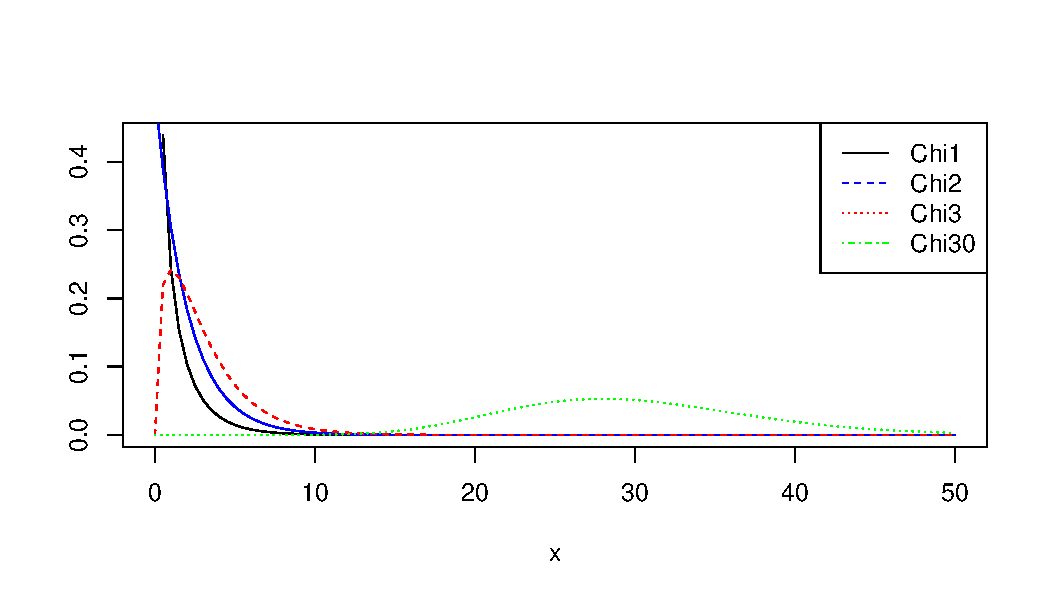
\includegraphics[width=\maxwidth]{figure/unnamed-chunk-5-1} 

\end{knitrout}
\end{frame}


\subsection[GoodnessofFit]{Steps for the Chi-Squared Test}
\begin{frame}[fragile]{Steps for the Chi-Squared Test}

\framebox{Context}
Consider a set of categorical data with $g$ categories in which fall observed counts $O_{i}$, for $i=1,2,\ldots,g$. A probability model is proposed for the categories, and we want to test whether it is adequate.

\vspace{.5cm}
\framebox{Preparation}
Construct the following table:

\begin{center}
\begin{tabular}{|l|lllll|l|} \hline
Class & 1 & 2 & 3 & \ldots & g & Totals \\ \hline
Observed Counts & $O_{1}$ & $O_{2}$ & $O_{3}$ & \ldots & $O_{g}$ & $\sum_{i=1}^{g} O_{i} = n$ \\
Expected Counts & $E_{1}$ & $E_{2}$ & $E_{3}$ & \ldots & $E_{g}$ & $\sum_{i=1}^{g} E_{i} = n$ \\ \hline
\end{tabular}
\end{center}

\vspace{.5cm}
Notes:
\begin{itemize}
\item $O_{i}$ are given, and $E_{i}$ need to be worked out from the hypothesised model $H_{0}$, so   $E_{i} = n P(category \;\; i)$.
\item Sometimes we need to estimate $k$ parameter(s) of the model first, before we can work out $E_{i}$.
\end{itemize}
\end{frame} 


\begin{frame}[fragile]{}

\framebox{H} $H_{0}$: Model fits. vs $H_{1}$: Model doesn't fit. \\

\framebox{A} Cochran's Rule: Check that $E_{i} \geq 1$ and no more than 20\% of $E_{i}$ are less than 5. If some of the $E_{i}$ are too small, then we combine categories together.

\framebox{T} 
\begin{itemize}
\item Definition Formula: $\tau = \sum_{i=1}^{g} \frac{(O_{i} - E_{i})^2}{E_{i}} \sim \chi^2_{g-k-1}$ (under $H_{0}$)
\item Calculation Formula: $\tau = \sum_{i=1}^{g} \frac{O_{i}^2}{E_{i}} - n \sim \chi^2_{g-k-1}$ (under $H_{0}$)
\item Large values of $\tau$ will argue against $H_{0}$ for $H_{1}$. \\  
(This indicates a difference between $O_{i}$ and $E_{i}$.)
\item The observed value is $\tau_{0}$. 
\end{itemize}

\framebox{P} $P$-value = $P( \chi^2_{g-k-1} \geq \tau_{0})$.

\framebox{C} Weigh up the $P$-value.
\end{frame}  


\subsection[GoodnessofFit]{Worked Examples}
\begin{frame}[fragile]{Example: Mendel's Early Genetics Model}

\framebox{Preparation}
Construct the following table:

\begin{center}
\begin{tabular}{|l|llll|l|} \hline
Class & RY & RG & AY & AG  & Totals \\ \hline
Observed Counts & 315  & 108 & 101 & 32 & 556 \\
Expected Counts & 312.75   & 104.25  & 104.25  & 34.75  & 556 \\ \hline
\end{tabular}
\end{center}

where: \\
$E_{1} = \frac{9}{9+3+3+1}*556 = \frac{9}{16}*556 = 312.75$ \\
$E_{2} = E_{3} =  \frac{3}{16}*556  = 104.25$. \\
$E_{4} = \frac{1}{16}*556  = 34.75$.\\

So the parameters are: $g=4, k=0$.
\end{frame} 

\begin{frame}[fragile]{}

\framebox{H} $H_{0}$: Model 9:3:3:1 fits. vs $H_{1}$: Model doesn't fit. \\

\framebox{A} Cochran's Rule: All $E_{i} \geq 1$ and no more than 20\% of $E_{i}$ are less than 5. 

\framebox{T} 
\begin{itemize}
\item Calculation Formula: $\tau = \sum_{i=1}^{4} \frac{O_{i}^2}{E_{i}} - 556 \sim \chi^2_{3}$ (under $H_{0}$)
\item Large values of $\tau$ will argue against $H_{0}$ for $H_{1}$, as this indicates a difference between $O_{i}$ and $E_{i}$.)
\item The observed value is $\tau_{0} = \frac{315^2}{312.75} + \frac{108^2}{104.25} + \frac{101^2}{104.25} + \frac{32^2}{34.75} - 556 \approx 0.47$. 
\end{itemize}

\begin{knitrout}
\definecolor{shadecolor}{rgb}{0.969, 0.969, 0.969}\color{fgcolor}\begin{kframe}
\begin{alltt}
\hlstd{o}\hlkwb{=}\hlkwd{c}\hlstd{(}\hlnum{315}\hlstd{,}\hlnum{108}\hlstd{,}\hlnum{101}\hlstd{,}\hlnum{32}\hlstd{)}
\hlstd{e}\hlkwb{=}\hlkwd{c}\hlstd{(}\hlnum{312.75}\hlstd{,}\hlnum{104.25}\hlstd{,}\hlnum{104.25}\hlstd{,}\hlnum{34.75}\hlstd{)}
\hlkwd{sum}\hlstd{((o}\hlopt{-}\hlstd{e)}\hlopt{^}\hlnum{2}\hlopt{/}\hlstd{e)}
\end{alltt}
\begin{verbatim}
## [1] 0.470024
\end{verbatim}
\begin{alltt}
\hlkwd{sum}\hlstd{(o}\hlopt{^}\hlnum{2}\hlopt{/}\hlstd{e)} \hlopt{-} \hlnum{556}
\end{alltt}
\begin{verbatim}
## [1] 0.470024
\end{verbatim}
\end{kframe}
\end{knitrout}
\end{frame}  


\begin{frame}[fragile]{}
\framebox{P} $P$-value = $P( \chi^2_{3} \geq 0.47) > 0.25 $ using tables.

\begin{knitrout}
\definecolor{shadecolor}{rgb}{0.969, 0.969, 0.969}\color{fgcolor}\begin{kframe}
\begin{alltt}
\hlnum{1}\hlopt{-}\hlkwd{pchisq}\hlstd{(}\hlnum{0.47}\hlstd{,}\hlnum{3}\hlstd{)}
\end{alltt}
\begin{verbatim}
## [1] 0.9254311
\end{verbatim}
\end{kframe}
\end{knitrout}


\framebox{C} As the $P$-value is so large, the data is consistent with Mendel's model.
\end{frame}  


\begin{frame}[fragile]{Example2: Random Number Generator}

\framebox{Preparation}
Construct the following table:

\vspace{.5cm}
{\tiny 
\begin{tabular}{l|llllllll}  \hline
Cat. & [0,0.1) &  [0.1,0.2) & [0.2,0.3) & [0.3,0.4) & [0.4,0.5) & [0.5,0.6) & [0.6,0.7) & [0.7,0.8)  \\ \hline
$O_{i}$ & 136 & 105 & 107 & 89 & 97 & 84 & 76 & 84    \\ \hline
$E_{i}$ & 100 & 100 & 100 & 100 & 100 & 100 & 100 & 100    \\ \hline
\end{tabular}
}

\vspace{.5cm}
{\tiny 
\begin{tabular}{l|lll}  \hline
Cat. & [0.8,0.9) &  [0.9,1] & Total \\ \hline
$O_{i}$ & 105  & 117  & 1000      \\ \hline
$E_{i}$ & 100  & 100  & 1000      \\ \hline
\end{tabular}
} 

\vspace{.5cm}
as $E_{i} = 1000/10 = 100$ for $i=1,2,\ldots,10$. 

\vspace{.5cm}
So the parameters are: $g=10, k=0$.
\end{frame} 

\begin{frame}[fragile]{}

\framebox{H} $H_{0}$: U[0,1] Model fits. vs $H_{1}$: Model doesn't fit. \\

\framebox{A} Cochran's Rule: All $E_{i} \geq 1$ and no more than 20\% of $E_{i}$ are less than 5. 

\framebox{T} 
\begin{itemize}
\item Calculation Formula: $\tau = \sum_{i=1}^{10} \frac{O_{i}^2}{E_{i}} - 1000 \sim \chi^2_{9}$ (under $H_{0}$)
\item Large values of $\tau$ will argue against $H_{0}$ for $H_{1}$, as this indicates a difference between $O_{i}$ and $E_{i}$.)
\item The observed value is $\tau_{0} = \frac{136^2}{100} + \frac{105^2}{100} + \ldots \frac{117^2}{100} - 1000 = 29.02$. 
\end{itemize}

\begin{knitrout}
\definecolor{shadecolor}{rgb}{0.969, 0.969, 0.969}\color{fgcolor}\begin{kframe}
\begin{alltt}
\hlstd{o}\hlkwb{=}\hlkwd{c}\hlstd{(}\hlnum{136}\hlstd{,}\hlnum{105}\hlstd{,}\hlnum{107}\hlstd{,}\hlnum{89}\hlstd{,}\hlnum{97}\hlstd{,}\hlnum{84}\hlstd{,}\hlnum{76}\hlstd{,}\hlnum{84}\hlstd{,}\hlnum{105}\hlstd{,}\hlnum{117}\hlstd{)}
\hlstd{e}\hlkwb{=}\hlkwd{c}\hlstd{(}\hlnum{100}\hlstd{,}\hlnum{100}\hlstd{,}\hlnum{100}\hlstd{,}\hlnum{100}\hlstd{,}\hlnum{100}\hlstd{,}\hlnum{100}\hlstd{,}\hlnum{100}\hlstd{,}\hlnum{100}\hlstd{,}\hlnum{100}\hlstd{,}\hlnum{100}\hlstd{)}
\hlkwd{sum}\hlstd{((o}\hlopt{-}\hlstd{e)}\hlopt{^}\hlnum{2}\hlopt{/}\hlstd{e)}
\end{alltt}
\begin{verbatim}
## [1] 29.02
\end{verbatim}
\begin{alltt}
\hlkwd{sum}\hlstd{(o}\hlopt{^}\hlnum{2}\hlopt{/}\hlstd{e)} \hlopt{-} \hlnum{1000}
\end{alltt}
\begin{verbatim}
## [1] 29.02
\end{verbatim}
\end{kframe}
\end{knitrout}
\end{frame} 


\begin{frame}[fragile]{}
\framebox{P} $P$-value = $P( \chi^2_{9} \geq 29.02) < 0.01$ using tables.

\begin{knitrout}
\definecolor{shadecolor}{rgb}{0.969, 0.969, 0.969}\color{fgcolor}\begin{kframe}
\begin{alltt}
\hlnum{1}\hlopt{-}\hlkwd{pchisq}\hlstd{(}\hlnum{29.02}\hlstd{,}\hlnum{9}\hlstd{)}
\end{alltt}
\begin{verbatim}
## [1] 0.0006430267
\end{verbatim}
\end{kframe}
\end{knitrout}

\framebox{C} As the $P$-value is so small, the data is not consistent with random number generator.
\end{frame} 


\begin{frame}[fragile]{Example3: Testing Data fits a Binomial Model}

\framebox{Preparation}

\vspace{.5cm}
(1) Fit parameters \\
In order to fit a Binomial model, we need the 2 parameters $n$ and $p$. Given the outcomes $0,1,2,3$, we have $n=3$, but $p$ is not given, so we need to estimate it from the data using the formula
\[ \hat{p} = \frac{0 \times 19 + 1 \times 34 + 2 \times 27 + 3 \times 20}{3 \times 100} \approx 0.493   \]
The formula arises because 100 Bin(3,p) trials is equivalent to 300 Bernoulli(p) trials.

\begin{knitrout}
\definecolor{shadecolor}{rgb}{0.969, 0.969, 0.969}\color{fgcolor}\begin{kframe}
\begin{alltt}
\hlstd{x}\hlkwb{=}\hlkwd{c}\hlstd{(}\hlnum{0}\hlstd{,}\hlnum{1}\hlstd{,}\hlnum{2}\hlstd{,}\hlnum{3}\hlstd{)}
\hlstd{o}\hlkwb{=}\hlkwd{c}\hlstd{(}\hlnum{19}\hlstd{,}\hlnum{34}\hlstd{,}\hlnum{27}\hlstd{,}\hlnum{20}\hlstd{)}
\hlkwd{sum}\hlstd{(x}\hlopt{*}\hlstd{o)}\hlopt{/}\hlstd{(}\hlnum{3}\hlopt{*}\hlkwd{sum}\hlstd{(o))}
\end{alltt}
\begin{verbatim}
## [1] 0.4933333
\end{verbatim}
\end{kframe}
\end{knitrout}
\end{frame} 

\begin{frame}[fragile]{}
(2) Construct the following table:

\vspace{.5cm}
\begin{tabular}{l|llll|l} 
Category & 0 & 1 & 2 & 3 & Total  \\ \hline
$O_{i}$ & 19 & 34 & 27 & 20 & 100    \\ \hline
$E_{i}$ & 13.03 & 38.02 & 36.97 & 11.98 & 100    \\ \hline
\end{tabular}

\vspace{.5cm}
as $E_{i} = {3 \choose i} (0.493)^i (1-0.493)^{3-i} \times 100$ for $i=0,1,2,3$. 

\begin{knitrout}
\definecolor{shadecolor}{rgb}{0.969, 0.969, 0.969}\color{fgcolor}\begin{kframe}
\begin{alltt}
\hlkwd{dbinom}\hlstd{(x,}\hlnum{3}\hlstd{,}\hlnum{0.493}\hlstd{)}\hlopt{*}\hlnum{100}
\end{alltt}
\begin{verbatim}
## [1] 13.03238 38.01755 36.96775 11.98232
\end{verbatim}
\end{kframe}
\end{knitrout}

\vspace{.5cm}
So the parameters are: $g=4, k=1$.
\end{frame} 

\begin{frame}[fragile]{}

\framebox{H} $H_{0}$: Bin(3,p) Model fits. vs $H_{1}$: Model doesn't fit. \\

\framebox{A} Cochran's Rule: All $E_{i} \geq 1$ and no more than 20\% of $E_{i}$ are less than 5. 

\framebox{T} 
\begin{itemize}
\item Calculation Formula: $\tau = \sum_{i=0}^{3} \frac{O_{i}^2}{E_{i}} - 100 \sim \chi^2_{4-1-1} = \chi^2_{2}$ (under $H_{0}$)
\item Large values of $\tau$ will argue against $H_{0}$ for $H_{1}$, as this indicates a difference between $O_{i}$ and $E_{i}$.
\item The observed value is $\tau_{0} = \frac{19^2}{13.03}  + \ldots \frac{20^2}{11.98} - 100 \approx 11.2$. 
\end{itemize}

{\tiny
\begin{knitrout}
\definecolor{shadecolor}{rgb}{0.969, 0.969, 0.969}\color{fgcolor}\begin{kframe}
\begin{alltt}
\hlstd{o}\hlkwb{=}\hlkwd{c}\hlstd{(}\hlnum{19}\hlstd{,}\hlnum{34}\hlstd{,}\hlnum{27}\hlstd{,}\hlnum{20}\hlstd{)}
\hlstd{e}\hlkwb{=}\hlkwd{c}\hlstd{(}\hlnum{13}\hlstd{,}\hlnum{38}\hlstd{,}\hlnum{37}\hlstd{,}\hlnum{12}\hlstd{)}
\hlkwd{sum}\hlstd{((o}\hlopt{-}\hlstd{e)}\hlopt{^}\hlnum{2}\hlopt{/}\hlstd{e)}
\end{alltt}
\begin{verbatim}
## [1] 11.22632
\end{verbatim}
\begin{alltt}
\hlkwd{sum}\hlstd{(o}\hlopt{^}\hlnum{2}\hlopt{/}\hlstd{e)} \hlopt{-} \hlnum{100}
\end{alltt}
\begin{verbatim}
## [1] 11.22632
\end{verbatim}
\end{kframe}
\end{knitrout}
}
\end{frame}  


\begin{frame}[fragile]{}
\framebox{P} $P$-value = $P( \chi^2_{2} \geq 11.2) < 0.01$ using tables.

\begin{knitrout}
\definecolor{shadecolor}{rgb}{0.969, 0.969, 0.969}\color{fgcolor}\begin{kframe}
\begin{alltt}
\hlnum{1}\hlopt{-}\hlkwd{pchisq}\hlstd{(}\hlnum{11.2}\hlstd{,}\hlnum{2}\hlstd{)}
\end{alltt}
\begin{verbatim}
## [1] 0.003697864
\end{verbatim}
\end{kframe}
\end{knitrout}

\framebox{C} As the $P$-value is so small, the data is not consistent with a Bin(3,p) model.

\vspace{.5cm}
Extension:
$X \sim \chi^2_{2} =  \exp(-\frac{x}{2})$, where
\[ P(X  \geq x) = e^{-\frac{x}{2}} \]
so the exact $P$-value is
\[ P( \chi^2_{2} \geq 11.2) = e^{-\frac{11.2}{2}} = 0.003697864 \]
\end{frame}  

\begin{frame}[fragile]{Example4: Testing Data fits a Normal Model}

This is a harder problem, as to fit a Normal distribution we need to estimate the 2 parameters: $\mu$ and $\sigma^2$. 

\vspace{.5cm}
We present a summarised solution, and then show how it could be done in R (Extension). 

{\tiny
\begin{knitrout}
\definecolor{shadecolor}{rgb}{0.969, 0.969, 0.969}\color{fgcolor}
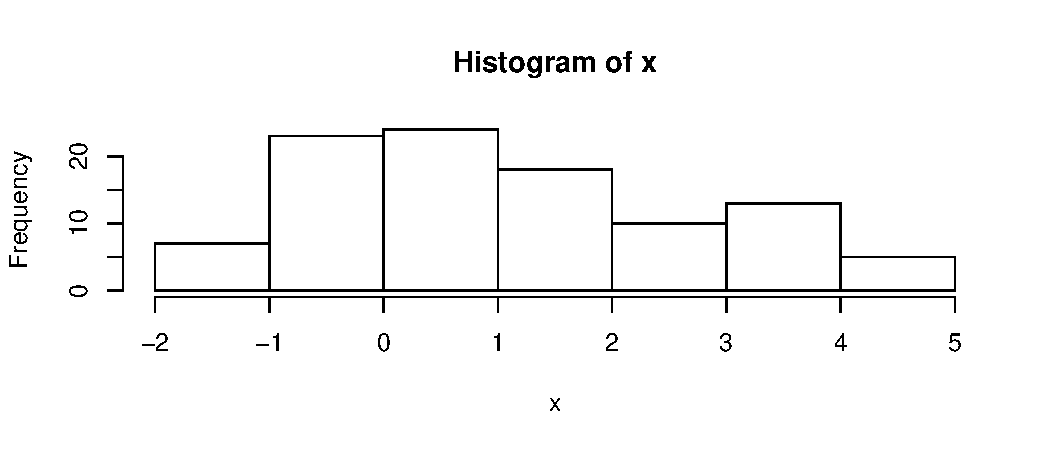
\includegraphics[width=\maxwidth]{figure/unnamed-chunk-14-1} 

\end{knitrout}
}
\end{frame}

\begin{frame}[fragile]{}
\framebox{Preparation}

\vspace{.5cm}
(1) To fit the 2 parameters, we divide the continuous data into categories, by finding out how many observations fit in each class of the histogram.

\vspace{.5cm}
\begin{tabular}{l|lllllll|l} 
Class & [-2,-1) & [-1,0) & [0,1) & [1,2) & [2,3) & [3,4) & [4,5) & Total  \\ \hline
$O_{i}$ & 7 & 23 & 24 & 18 & 10 & 13 & 5 & 100    \\ \hline
\end{tabular}

\vspace{.5cm}
To work out the mean, we use the midpoint of each class as an estimate of the obervations in that class.
So the 1st class has 7 observations in [-2,-1) each approximated by -1.5. 

\vspace{.5cm}
Hence the mean estimate is 
{\tiny
\[ \hat{\mu} = \frac{7 \times (-1.5) + 23 \times (-0.5) + 24 \times (0.5) + 18 \times 1.5 + 10 \times 2.5 + 13 \times 3.5 + 5 \times 4.5}{100} = 1.1 \]
}
\end{frame}

\begin{frame}[fragile]{}

Similarly, we can work out the variance

{\tiny
\[ \hat{\sigma^2} = \frac{7 \times (-1.5)^2 + 23 \times(-0.5)^2 + 24 \times (0.5)^2 + \ldots + 5 \times 4.5^2 - 100 \times (1.1)^2}{99} = 2.727273 \]
}
So 
\[ \hat{\sigma} = \sqrt{2.727273} \approx 1.65 \]

Therefore, for fitting the Normal we use the 2 parameters: $\mu = 1.1$ and $\sigma = 1.65$.

\vspace{.5cm}
Note that we based these estimates on the grouped data, not the original ungrouped data. If we used the ungrouped data we would get a larger statistic and so a misleading small $P$-value.
\end{frame}

\begin{frame}[fragile]{}

(2) Work out the Expected Values for $N(1.1,1.65^2)$.

\vspace{.5cm}
Note: We now change the first interval to $(-\infty,-1)$ and last to $[4,\infty)$, to be consistent with the Normal which spans $(-\infty,\infty)$.

\vspace{.5cm}
We construct the following table:

\vspace{.5cm}
\begin{tabular}{l|lllllll|l} 
Class & (-$\infty$,-1) & [-1,0) & [0,1) & [1,2) & [2,3) & [3,4) & [4,$\infty$) & Total  \\ \hline
$O_{i}$ & 7 & 23 & 24 & 18 & 10 & 13 & 5 & 100    \\ \hline
$E_{i}$ & 10.16 & 15.09 & 22.33 & 23.14 & 16.80 & 8.54 & 3.94 & 100    \\ \hline
\end{tabular}

\vspace{.5cm}
where the Expected Counts in (-$\infty$,-1) = 10.16
\begin{knitrout}
\definecolor{shadecolor}{rgb}{0.969, 0.969, 0.969}\color{fgcolor}\begin{kframe}
\begin{alltt}
\hlkwd{pnorm}\hlstd{(}\hlopt{-}\hlnum{1}\hlstd{,}\hlnum{1.1}\hlstd{,}\hlnum{1.65}\hlstd{)}\hlopt{*}\hlnum{100}
\end{alltt}
\begin{verbatim}
## [1] 10.15574
\end{verbatim}
\end{kframe}
\end{knitrout}
\end{frame}

\begin{frame}[fragile]{}
and the Expected Counts in [-1,0) = 15.09
\begin{knitrout}
\definecolor{shadecolor}{rgb}{0.969, 0.969, 0.969}\color{fgcolor}\begin{kframe}
\begin{alltt}
\hlstd{(}\hlkwd{pnorm}\hlstd{(}\hlnum{0}\hlstd{,}\hlnum{1.1}\hlstd{,}\hlnum{1.65}\hlstd{)}\hlopt{-}\hlkwd{pnorm}\hlstd{(}\hlopt{-}\hlnum{1}\hlstd{,}\hlnum{1.1}\hlstd{,}\hlnum{1.65}\hlstd{))}\hlopt{*}\hlnum{100}
\end{alltt}
\begin{verbatim}
## [1] 15.09351
\end{verbatim}
\end{kframe}
\end{knitrout}

\vspace{.5cm}
Other values follow:
{\tiny
\begin{knitrout}
\definecolor{shadecolor}{rgb}{0.969, 0.969, 0.969}\color{fgcolor}\begin{kframe}
\begin{alltt}
\hlstd{(}\hlkwd{pnorm}\hlstd{(}\hlnum{1}\hlstd{,}\hlnum{1.1}\hlstd{,}\hlnum{1.65}\hlstd{)}\hlopt{-}\hlkwd{pnorm}\hlstd{(}\hlnum{0}\hlstd{,}\hlnum{1.1}\hlstd{,}\hlnum{1.65}\hlstd{))}\hlopt{*}\hlnum{100}
\end{alltt}
\begin{verbatim}
## [1] 22.33439
\end{verbatim}
\begin{alltt}
\hlstd{(}\hlkwd{pnorm}\hlstd{(}\hlnum{2}\hlstd{,}\hlnum{1.1}\hlstd{,}\hlnum{1.65}\hlstd{)}\hlopt{-}\hlkwd{pnorm}\hlstd{(}\hlnum{1}\hlstd{,}\hlnum{1.1}\hlstd{,}\hlnum{1.65}\hlstd{))}\hlopt{*}\hlnum{100}
\end{alltt}
\begin{verbatim}
## [1] 23.14431
\end{verbatim}
\begin{alltt}
\hlstd{(}\hlkwd{pnorm}\hlstd{(}\hlnum{3}\hlstd{,}\hlnum{1.1}\hlstd{,}\hlnum{1.65}\hlstd{)}\hlopt{-}\hlkwd{pnorm}\hlstd{(}\hlnum{2}\hlstd{,}\hlnum{1.1}\hlstd{,}\hlnum{1.65}\hlstd{))}\hlopt{*}\hlnum{100}
\end{alltt}
\begin{verbatim}
## [1] 16.79603
\end{verbatim}
\end{kframe}
\end{knitrout}
}
\end{frame} 

\begin{frame}[fragile]{}

{\tiny 
\begin{knitrout}
\definecolor{shadecolor}{rgb}{0.969, 0.969, 0.969}\color{fgcolor}\begin{kframe}
\begin{alltt}
\hlstd{(}\hlkwd{pnorm}\hlstd{(}\hlnum{4}\hlstd{,}\hlnum{1.1}\hlstd{,}\hlnum{1.65}\hlstd{)}\hlopt{-}\hlkwd{pnorm}\hlstd{(}\hlnum{3}\hlstd{,}\hlnum{1.1}\hlstd{,}\hlnum{1.65}\hlstd{))}\hlopt{*}\hlnum{100}
\end{alltt}
\begin{verbatim}
## [1] 8.535032
\end{verbatim}
\begin{alltt}
\hlstd{(}\hlnum{1}\hlopt{-}\hlkwd{pnorm}\hlstd{(}\hlnum{4}\hlstd{,}\hlnum{1.1}\hlstd{,}\hlnum{1.65}\hlstd{))}\hlopt{*}\hlnum{100}
\end{alltt}
\begin{verbatim}
## [1] 3.940986
\end{verbatim}
\end{kframe}
\end{knitrout}
}

\vspace{.5cm}
So the parameters are: $g=7, k=2$.
\end{frame} 

\begin{frame}[fragile]{}

\framebox{H} $H_{0}$: $N(1.1,1.65^2)$ Model fits. vs $H_{1}$: Model doesn't fit. \\

\framebox{A} Cochran's Rule: All $E_{i} \geq 1$ and no more than 20\% of $E_{i}$ are less than 5. 

\framebox{T} 
\begin{itemize}
\item Calculation Formula: $\tau = \sum_{i=1}^{7} \frac{O_{i}^2}{E_{i}} - 100 \sim \chi^2_{7-1-2} = \chi^2_{4}$ (under $H_{0}$)
\item Large values of $\tau$ will argue against $H_{0}$ for $H_{1}$, as this indicates a difference between $O_{i}$ and $E_{i}$.)
\item The observed value is $\tau_{0} = \frac{7^2}{10.16} + \ldots \frac{5^2}{3.94} - 100 \approx 11.76$. 
\end{itemize}
\end{frame}  


\begin{frame}[fragile]{}
\framebox{P} $P$-value = $P( \chi^2_{4} \geq 11.76) \in (0.01,0.025) $ using tables.

\begin{knitrout}
\definecolor{shadecolor}{rgb}{0.969, 0.969, 0.969}\color{fgcolor}\begin{kframe}
\begin{alltt}
\hlnum{1}\hlopt{-}\hlkwd{pchisq}\hlstd{(}\hlnum{11.76}\hlstd{,}\hlnum{4}\hlstd{)}
\end{alltt}
\begin{verbatim}
## [1] 0.01922812
\end{verbatim}
\end{kframe}
\end{knitrout}

\framebox{C} As the $P$-value is small, the data are not consistent with a Normal model, as evident from the Normal curve on the histogram.


\begin{knitrout}
\definecolor{shadecolor}{rgb}{0.969, 0.969, 0.969}\color{fgcolor}
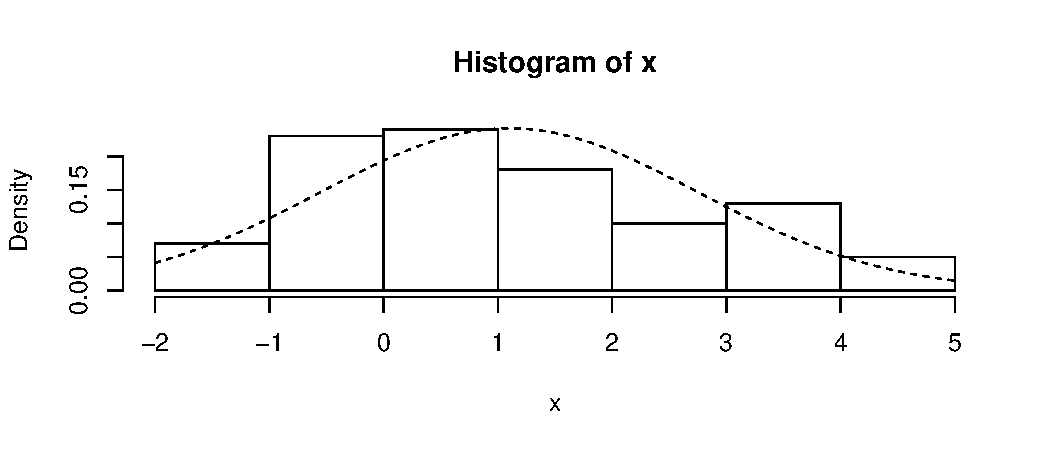
\includegraphics[width=\maxwidth]{figure/unnamed-chunk-20-1} 

\end{knitrout}

\end{frame} 



\begin{frame}[fragile]{Solving in R (Extension)}

\vspace{.5cm}
Note: These results differ a tiny bit, as previously we rounded the estimate of standard deviation to 2dp.

\vspace{.5cm}
(1) Scan data and produce histogram
{\tiny
\begin{knitrout}
\definecolor{shadecolor}{rgb}{0.969, 0.969, 0.969}\color{fgcolor}\begin{kframe}
\begin{alltt}
\hlstd{x} \hlkwb{<-} \hlkwd{read.table}\hlstd{(}\hlstr{"http://www.maths.usyd.edu.au/u/UG/JM/MATH1005/r/StatsData/w13.txt"}\hlstd{)}
\hlstd{x}\hlkwb{=}\hlkwd{unlist}\hlstd{(x)} \hlcom{#Changes data frame to vector}
\hlkwd{hist}\hlstd{(x)}
\end{alltt}
\end{kframe}
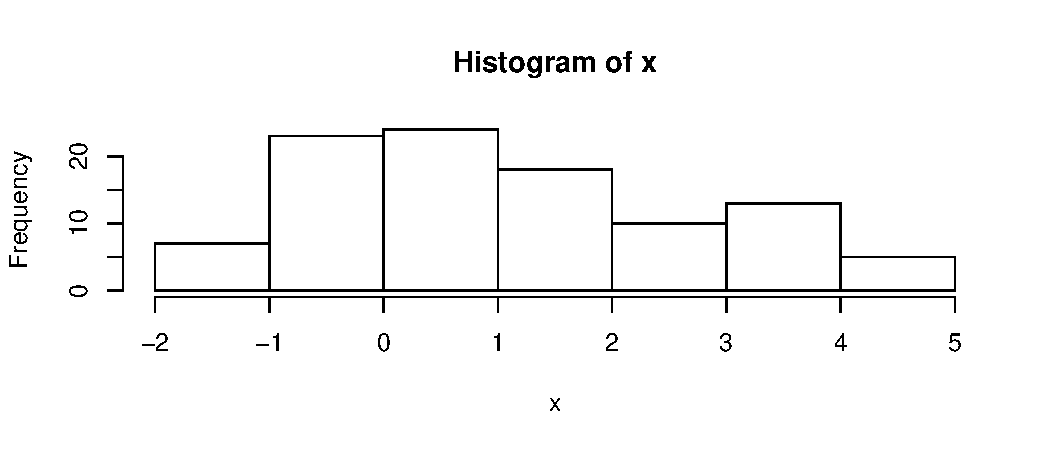
\includegraphics[width=\maxwidth]{figure/unnamed-chunk-21-1} 

\end{knitrout}
}

%\includegraphics[height=4cm]{Topic11_Q2.pdf}
\end{frame}





\begin{frame}[fragile]{}
(2) Find the Observed Counts, from a histogram of the data.

\begin{knitrout}
\definecolor{shadecolor}{rgb}{0.969, 0.969, 0.969}\color{fgcolor}\begin{kframe}
\begin{alltt}
\hlcom{#Lists the class breaks (-2,-1], (-1,0] etc}
\hlkwd{hist}\hlstd{(x,}\hlkwc{pr}\hlstd{=T)}\hlopt{$}\hlstd{breaks}
\end{alltt}
\begin{verbatim}
## [1] -2 -1  0  1  2  3  4  5
\end{verbatim}
\begin{alltt}
\hlstd{freq}\hlkwb{=}\hlkwd{hist}\hlstd{(x,}\hlkwc{pr}\hlstd{=T)}\hlopt{$}\hlstd{counts}  \hlcom{#Observed Counts O_i}
\end{alltt}
\end{kframe}
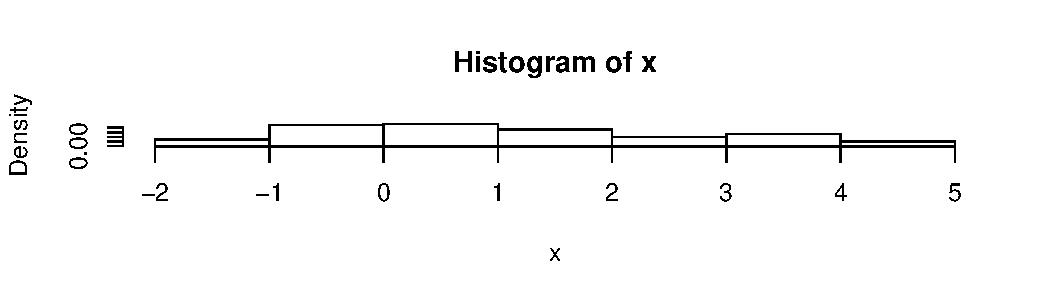
\includegraphics[width=\maxwidth]{figure/unnamed-chunk-22-1} 
\begin{kframe}\begin{alltt}
\hlstd{freq}
\end{alltt}
\begin{verbatim}
## [1]  7 23 24 18 10 13  5
\end{verbatim}
\end{kframe}
\end{knitrout}
\end{frame}

\begin{frame}[fragile]{}
(3) Estimate the 2 parameters of Normal: mean and sd.
\begin{knitrout}
\definecolor{shadecolor}{rgb}{0.969, 0.969, 0.969}\color{fgcolor}\begin{kframe}
\begin{alltt}
\hlstd{mids}\hlkwb{=}\hlstd{(}\hlopt{-}\hlnum{2}\hlopt{:}\hlnum{4}\hlstd{)}\hlopt{+}\hlnum{.5}    \hlcom{#Midpoints of each class}
\hlstd{mids}
\end{alltt}
\begin{verbatim}
## [1] -1.5 -0.5  0.5  1.5  2.5  3.5  4.5
\end{verbatim}
\begin{alltt}
\hlstd{gr.sum}\hlkwb{=}\hlkwd{sum}\hlstd{(freq}\hlopt{*}\hlstd{mids)}
\hlstd{gr.sum}
\end{alltt}
\begin{verbatim}
## [1] 110
\end{verbatim}
\begin{alltt}
\hlstd{gr.sumsq}\hlkwb{=}\hlkwd{sum}\hlstd{(freq}\hlopt{*}\hlstd{mids}\hlopt{^}\hlnum{2}\hlstd{)}
\hlstd{gr.sumsq}
\end{alltt}
\begin{verbatim}
## [1] 391
\end{verbatim}
\end{kframe}
\end{knitrout}
\end{frame}

\begin{frame}[fragile]{}
\begin{knitrout}
\definecolor{shadecolor}{rgb}{0.969, 0.969, 0.969}\color{fgcolor}\begin{kframe}
\begin{alltt}
\hlstd{gr.mean}\hlkwb{=}\hlstd{gr.sum}\hlopt{/}\hlnum{100}   \hlcom{#Estimate of mean}
\hlstd{gr.mean}
\end{alltt}
\begin{verbatim}
## [1] 1.1
\end{verbatim}
\begin{alltt}
\hlstd{gr.var}\hlkwb{=}\hlnum{1}\hlopt{/}\hlnum{99}\hlopt{*} \hlstd{(gr.sumsq} \hlopt{-} \hlnum{1}\hlopt{/}\hlnum{100}\hlopt{*} \hlstd{gr.sum}\hlopt{^}\hlnum{2}\hlstd{)}
\hlstd{gr.var}
\end{alltt}
\begin{verbatim}
## [1] 2.727273
\end{verbatim}
\begin{alltt}
\hlstd{gr.sd}\hlkwb{=}\hlkwd{sqrt}\hlstd{(gr.var)}   \hlcom{#Estimate of sd}
\hlstd{gr.sd}
\end{alltt}
\begin{verbatim}
## [1] 1.651446
\end{verbatim}
\end{kframe}
\end{knitrout}
\end{frame}

\begin{frame}[fragile]{}
(4) Find the Expected Counts, from fitting a $N(1.1, 1.651446^2)$ model.

\begin{knitrout}
\definecolor{shadecolor}{rgb}{0.969, 0.969, 0.969}\color{fgcolor}\begin{kframe}
\begin{alltt}
\hlcom{#Add Normal PDF to the histogram}
\hlkwd{hist}\hlstd{(x,} \hlkwc{pr}\hlstd{=T)}
\hlkwd{curve}\hlstd{(}\hlkwd{dnorm}\hlstd{(x,}\hlkwc{m}\hlstd{=gr.mean,}\hlkwc{s}\hlstd{=gr.sd),}\hlkwc{lty}\hlstd{=}\hlnum{2}\hlstd{,}\hlkwc{add}\hlstd{=T)}
\end{alltt}
\end{kframe}
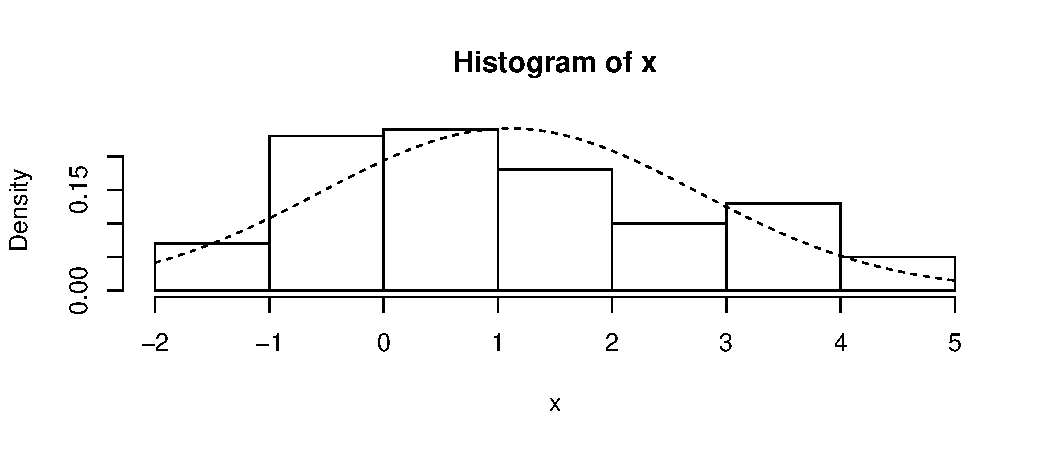
\includegraphics[width=\maxwidth]{figure/unnamed-chunk-25-1} 

\end{knitrout}
\end{frame}

\begin{frame}[fragile]{}
\begin{knitrout}
\definecolor{shadecolor}{rgb}{0.969, 0.969, 0.969}\color{fgcolor}\begin{kframe}
\begin{alltt}
\hlcom{#Normal probability at lower threshold of each interval}
\hlstd{lower.probs}\hlkwb{=}\hlkwd{pnorm}\hlstd{(}\hlopt{-}\hlnum{1}\hlopt{:}\hlnum{4}\hlstd{,}\hlkwc{m}\hlstd{=gr.mean,}\hlkwc{s}\hlstd{=gr.sd)}
\hlstd{lower.probs}
\end{alltt}
\begin{verbatim}
## [1] 0.1017553 0.2526790 0.4758576 0.7071154 0.8750325 0.9604590
\end{verbatim}
\begin{alltt}
\hlcom{#The probability in each interval (upper-lower)}
\hlstd{exp.probs}\hlkwb{=}\hlkwd{diff}\hlstd{(}\hlkwd{c}\hlstd{(}\hlnum{0}\hlstd{,lower.probs,}\hlnum{1}\hlstd{))}
\hlstd{exp.probs}
\end{alltt}
\begin{verbatim}
## [1] 0.10175530 0.15092370 0.22317860 0.23125775 0.16791712 0.08542650
## [7] 0.03954103
\end{verbatim}
\begin{alltt}
\hlcom{#Find Expected frequencies/counts E_i}
\hlstd{exp.freq}\hlkwb{=} \hlnum{100}\hlopt{*} \hlstd{exp.probs}
\hlstd{exp.freq}
\end{alltt}
\begin{verbatim}
## [1] 10.175530 15.092370 22.317860 23.125775 16.791712  8.542650  3.954103
\end{verbatim}
\end{kframe}
\end{knitrout}
\end{frame}

\begin{frame}[fragile]{}
(5) Calculate the chi-squared test statistic, and $P$-value.
\begin{knitrout}
\definecolor{shadecolor}{rgb}{0.969, 0.969, 0.969}\color{fgcolor}\begin{kframe}
\begin{alltt}
\hlcom{#Find Chi-squared contributions}
\hlstd{contrib} \hlkwb{=} \hlstd{((exp.freq}\hlopt{-}\hlstd{freq)}\hlopt{^}\hlnum{2}\hlstd{)}\hlopt{/}\hlstd{exp.freq}
\hlstd{contrib}
\end{alltt}
\begin{verbatim}
## [1] 0.9910041 4.1431939 0.1267861 1.1361164 2.7470308 2.3257383 0.2766496
\end{verbatim}
\begin{alltt}
\hlcom{# Put O-i, E_i, Chi-Sq in table}
\hlkwd{cbind}\hlstd{(freq,exp.freq,contrib)}
\end{alltt}
\begin{verbatim}
##      freq  exp.freq   contrib
## [1,]    7 10.175530 0.9910041
## [2,]   23 15.092370 4.1431939
## [3,]   24 22.317860 0.1267861
## [4,]   18 23.125775 1.1361164
## [5,]   10 16.791712 2.7470308
## [6,]   13  8.542650 2.3257383
## [7,]    5  3.954103 0.2766496
\end{verbatim}
\end{kframe}
\end{knitrout}
\end{frame}

\begin{frame}[fragile]{}
\begin{knitrout}
\definecolor{shadecolor}{rgb}{0.969, 0.969, 0.969}\color{fgcolor}\begin{kframe}
\begin{alltt}
\hlcom{#Calculate Chi-squared test statistic}
\hlstd{tau.obs}\hlkwb{=}\hlkwd{sum}\hlstd{(((exp.freq}\hlopt{-}\hlstd{freq)}\hlopt{^}\hlnum{2}\hlstd{)}\hlopt{/}\hlstd{exp.freq)}
\hlstd{tau.obs}
\end{alltt}
\begin{verbatim}
## [1] 11.74652
\end{verbatim}
\begin{alltt}
\hlcom{#Calculate P-value}
\hlnum{1}\hlopt{-}\hlkwd{pchisq}\hlstd{(tau.obs,} \hlkwc{df}\hlstd{=}\hlkwd{length}\hlstd{(freq)}\hlopt{-}\hlnum{2}\hlopt{-}\hlnum{1}\hlstd{)}
\end{alltt}
\begin{verbatim}
## [1] 0.0193392
\end{verbatim}
\end{kframe}
\end{knitrout}
\end{frame}


\end{document}
